\documentclass[../main.tex]{subfiles}

\usepackage{nopageno} %Seitenzahlen auf richtiger Seite 

\usepackage[left=2cm, right=2cm, top=2cm, includehead, includefoot, headheight=17pt]{geometry}

\usepackage[utf8x]{inputenc}
\usepackage[english]{babel}
\usepackage{amsmath,amssymb,amsthm}
\usepackage{framed}
\usepackage{wasysym}
\usepackage[T1]{fontenc} %Silbentrennung 
\usepackage{color} %Farbe
\usepackage{graphicx}
\usepackage{float}%Grafik am gleichen Ort plazieren
%pdf. png. einfach eingliedern
\usepackage{subfigure} %Grafiken nebeneinander
\usepackage{pdfpages}
\usepackage{ulem} 	%\uuline{urgent}    % doppelt unterstreichen
%\uwave{boat}      % unterschlängeln
%\sout{wrong}       % durchstreichen
%\xout{removed}     % ausstreichen mit //////.

\usepackage{tikz}
\usetikzlibrary{trees}
\usetikzlibrary{plotmarks}
\usetikzlibrary{angles,quotes,babel}
\usetikzlibrary{shadings}
\usetikzlibrary{patterns}
\usetikzlibrary{matrix}
\usetikzlibrary{arrows}
\usetikzlibrary{calc}

\usepackage{pgfplots}
\usepackage{pgf-pie}
\pgfplotsset{compat=1.10}
\usepgfplotslibrary{statistics}
\usepgfplotslibrary{fillbetween}

\usepackage{tkz-euclide}
\usepackage{enumerate}
\usepackage{stmaryrd}
\usepackage{tabularx}
\usepackage{wrapfig}
\usepackage{epsdice}
\usepackage{multirow}
\usepackage{rotating}
\usepackage{pdflscape}
\usepackage{fancyhdr}

\pagestyle{fancy} %eigener Seitenstil
\fancyhf{} %alle Kopf- und Fußzeilenfelder bereinigen
\fancyhead[L]{} %Kopfzeile links
\fancyhead[C]{} %zentrierte Kopfzeile
\fancyhead[R]{} %Kopfzeile rechts
\renewcommand{\headrulewidth}{0.4pt} %obere Trennlinie
\fancyfoot[C]{\thepage} %Seitennummer
\renewcommand{\footrulewidth}{0.4pt} %untere Trennlinie

% Number spaces 
\newcommand{\CC}{\ensuremath{\mathbb{C}}}
\newcommand{\RR}{\ensuremath{\mathbb{R}}}
\newcommand{\QQ}{\ensuremath{\mathbb{Q}}}
\newcommand{\ZZ}{\ensuremath{\mathbb{Z}}}
\newcommand{\NN}{\ensuremath{\mathbb{N}}}
\newcommand{\LL}{\ensuremath{\mathbb{L}}}
\newcommand{\DD}{\ensuremath{\mathbb{D}}}
\newcommand{\WW}{\ensuremath{\mathbb{W}}}

%draw chemestry molecules 
\usepackage{chemfig} % https://mirror.ox.ac.uk/sites/ctan.org/macros/generic/chemfig/

\newcommand\vv[1]{%
	\begin{tikzpicture}[baseline=(arg.base)]
		\node[inner xsep=0pt] (arg) {$#1$};
		\draw[line cap=round,line width=0.45,->,shorten >= 0.2pt, shorten <= 0.7pt] (arg.north west) -- (arg.north east);
	\end{tikzpicture}%
} %command will render \vv{x} with an arrow aboth 

\renewcommand{\labelenumi}{\roman{enumi})}

\DeclareMathOperator{\ggT}{ggT}
\DeclareMathOperator{\sign}{sign}

%sections
\theoremstyle{plain}
\newtheorem{Thm}{Theorem}[section]
\newtheorem{Def}[Thm]{Definition}
\newtheorem{Prop}[Thm]{Proposition}

\theoremstyle{definition}
\newtheorem{lemma}[Thm]{Lemma}
\newtheorem{corollary}[Thm]{Corollary}
\newtheorem{claim}[Thm]{Claim}
\newtheorem{Proof}[Thm]{Proof}
\newtheorem{Ex}[Thm]{Example}

\newtheorem{Exercise}{ex}[section] %follow proper enum
\newtheorem{ex}[Exercise]{Exercise}
\newtheorem{Solution}{sol}[section]
\newtheorem{sol}[Solution]{Solution}

\theoremstyle{remark}
\newtheorem{remark}[Thm]{Remark} % follows thm enum

\newtheorem{comment}{Comment}[section] %follow comment enum
\newtheorem{notation}[comment]{Notation}
\newtheorem{reasoning}[comment]{Reasoning}
\newtheorem{Intpr}[comment]{Interpretation}

%some premmade with title (uterwise use \textbf{Title} ...)
\newenvironment{ThmWithTitle}[1]{%
	\begin{Thm}[\textbf{#1}]}{\end{Thm}}
\newenvironment{PropWithTitle}[1]{%
	\begin{Prop}[\textbf{#1}]}{\end{Prop}}
\newenvironment{ExWithTitle}[1]{%
	\begin{Ex}[\textbf{#1}]}{\end{Ex}}
\newenvironment{DefWithTitle}[1]{%
	\begin{Def}[\textbf{#1}]}{\end{Def}}
\newenvironment{RemarkWithTitel}[1]{%
	\begin{remark}[\textbf{#1}]}{\end{remark}}

%format of paragraph 
\renewcommand\paragraph{\@startsection{paragraph}{4}{\z@}%
	{-2.5ex\@plus -1ex \@minus -.25ex}%
	{1.25ex \@plus .25ex}%
	{\normalfont\normalsize\bfseries}}
\makeatother
\setcounter{secnumdepth}{4} % how many sectioning levels to assign numbers to
\setcounter{tocdepth}{4}    % how many sectioning levels to show in ToC

\newcounter{row} 
\renewcommand\therow{\alph{row}} %hier a,b,c etc. def und mit therow abrufbar

\newenvironment{aufz}
{\setcounter{row}{0}%
	\par\noindent\tabularx{\linewidth}[t]
	{\cdot{20}{>{\stepcounter{row}\makebox[1.5em][l]{\therow)\hfill}}X}} %bis max 20 Elemente nebeinander
}
{\endtabularx}


%biblio
\usepackage[]{biblatex}
\addbibresource{referenzenma.bib} 

%glossary
\usepackage{glossaries}
\usepackage{import}


\usepackage{rotating} % Include this package in the preamble

\newglossaryentry{anabolism}{
	name={Anabolism},
	description={Metabolic pathways that build complex molecules from simpler ones, requiring an input of energy.}
}

\newglossaryentry{atp}{
	name={ATP (Adenosine Triphosphate)},
	description={The primary energy currency of the cell, used to power many cellular processes. Its hydrolysis releases heat but not energy, while the transfer of phosphate leads to a higher state in free energy of the substrate.}
}

\newglossaryentry{catabolism}{
	name={Catabolism},
	description={Metabolic pathways that break down complex molecules into simpler ones, releasing energy.}
}

\newglossaryentry{coupledreactions}{
	name={Coupled Reactions},
	description={Two chemical reactions linked together, where an energetically favourable reaction (e.g., ATP hydrolysis) provides the energy to drive an energetically unfavourable reaction.}
}

\newglossaryentry{electroncarrier}{
	name={Electron Carrier},
	description={Molecules that can accept and donate electrons, facilitating the transfer of energy in redox reactions (e.g., NAD+, FAD).}
}

\newglossaryentry{glycolysis}{
	name={Glycolysis},
	description={A universal metabolic pathway that breaks down glucose into pyruvate, producing a net gain of ATP and NADH.}
}

\newglossaryentry{metabolism}{
	name={Metabolism},
	description={The sum of all chemical reactions that occur within a living organism to maintain life.}
}

\newglossaryentry{oxidation}{
	name={Oxidation},
	description={The loss of electrons or an increase in oxidation state of a molecule. Often involves the addition of oxygen or removal of hydrogen.}
}

\newglossaryentry{phosphorylation}{
	name={Phosphorylation},
	description={The addition of a phosphate group to a molecule, often increasing its energy or altering its activity.}
}


\newglossaryentry{reduction}{
	name={Reduction},
	description={The gain of electrons or a decrease in oxidation state of a molecule. Often involves the addition of hydrogen or removal of oxygen.}
}

\newglossaryentry{secondlaw}{
	name={Second Law of Thermodynamics},
	description={States that the total entropy of an isolated system can never decrease over time.}
}

\newglossaryentry{enthalpy}{
	name={Enthalpy (H)},
	description={A thermodynamic quantity representing the total heat content of a system. In biochemistry, enthalpy changes (\(\Delta H\)) are associated with bond formation and breaking, influencing biochemical reactions and energy transfer.}
}

\newglossaryentry{entropy}{
	name={Entropy},
	description={A measure of the disorder or randomness of a system. The second law of thermodynamics states that the total entropy of an isolated system tends to increase over time.}
}

\newglossaryentry{exergonicreaction}{
	name={Exergonic Reaction},
	description={A chemical reaction that releases energy (has a negative \( \Delta G \)) and is therefore favorable. }
}

\newglossaryentry{freeenergy}{
	name={Free Energy (G)},
	description={The portion of a system's energy that is available to do useful work.}
}


\newglossaryentry{kinase}{
	name={Kinase},
	description={An enzyme that catalyzes the transfer of phosphate groups from high-energy donor molecules, such as ATP, to specific substrates, a process known as phosphorylation.}
}

\newglossaryentry{phosphatase}{
	name={Phosphatase},
	description={An enzyme that removes phosphate groups from proteins or other molecules, a process known as dephosphorylation, which often regulates cellular activity.}
}

\newglossaryentry{dehydrogenase}{
	name={Dehydrogenase},
	description={An enzyme that catalyzes the removal of two hydrogen atoms from a substrate, typically transferring them to an electron acceptor such as NAD$^+$ or FAD. Dehydrogenases play a crucial role in metabolic pathways like glycolysis and the citric acid cycle.}
}

\newglossaryentry{oxidase}{
	name={Oxidase},
	description={An enzyme that catalyzes oxidation reactions, using molecular oxygen (O$_2$) as the electron acceptor without incorporating it into the substrate. Oxidases are involved in various biological oxidation processes, including those in the electron transport chain.}
}

\newglossaryentry{oxygenase}{
	name={Oxygenase},
	description={An enzyme that catalyzes the incorporation of oxygen atoms from molecular oxygen (O$_2$) into a substrate. Oxygenases are classified into monooxygenases and dioxygenases, which incorporate one or two oxygen atoms, respectively, and are essential in metabolic pathways like drug metabolism and biosynthesis.}
}

\newglossaryentry{reducingequivalent}{
	name={Reducing Equivalent},
	description={A unit of reducing power in biochemical redox reactions, referring to the transfer of one electron (or its equivalent as a hydrogen atom or hydride ion). Reducing equivalents are carried by molecules such as NADH, NADPH, and FADH$_2$, playing a crucial role in cellular respiration and biosynthetic pathways.}
}

\newglossaryentry{niacin}{
	name={Niacin (Vitamin B3)},
	description={A water-soluble B vitamin essential for energy metabolism, DNA repair, and cell signaling. Niacin is a precursor to the coenzymes NAD$^+$ and NADP$^+$, which are crucial for redox reactions in cellular respiration and biosynthetic pathways}
}

\newglossaryentry{arsenatepoisoning}{
	name={Arsenate Poisoning},
	description={A toxic condition caused by exposure to arsenate (AsO$_4^{3-}$), which disrupts cellular metabolism by mimicking phosphate. Arsenate can uncouple oxidative phosphorylation by substituting for inorganic phosphate glycolisys or ATP synthesis, leading to decreased ATP production and cellular toxicity. Symptoms include nausea, vomiting, neurological disturbances, and multi-organ failure in severe cases.}
}

\newglossaryentry{nad}{
	name={NAD$^+$ (Nicotinamide Adenine Dinucleotide)},
	description={A coenzyme involved in redox reactions, serving as an electron carrier in cellular respiration. NAD$^+$ is reduced to NADH, which donates electrons to the electron transport chain for ATP production.}
}

\newglossaryentry{nadp}{
	name={NADP$^+$ (Nicotinamide Adenine Dinucleotide Phosphate)},
	description={A phosphorylated form of NAD$^+$ that functions as an electron carrier, primarily in anabolic pathways such as fatty acid and nucleotide biosynthesis. NADP$^+$ is reduced to NADPH, which provides reducing power for biosynthetic reactions.}
}

\newglossaryentry{fad}{
	name={FAD (Flavin Adenine Dinucleotide)},
	description={A redox-active coenzyme associated with various enzymes, particularly in the electron transport chain and fatty acid oxidation. FAD is reduced to FADH$_2$, which donates electrons to the respiratory chain.}
}

\newglossaryentry{fmn}{
	name={FMN (Flavin Mononucleotide)},
	description={A coenzyme derived from riboflavin (vitamin B2) that acts as a prosthetic group in various oxidoreductases, including NADH dehydrogenase in the electron transport chain. FMN is involved in redox reactions, cycling between oxidized and reduced states.}
}


\newglossaryentry{flavoprotein}{
	name={Flavoprotein},
	description={A protein that contains a flavin coenzyme, such as FAD or FMN, as a prosthetic group}
}

\newglossaryentry{ubiquinone}{
	name={Ubiquinone (Coenzyme Q)},
	description={A lipid-soluble electron carrier in the electron transport chain, transferring electrons between complex I/II and complex III. Ubiquinone exists in oxidized (Q), semiquinone (Q$^-$), and reduced (QH$_2$) forms.}
}



\makeglossaries

\begin{document}

\section{Behind the Torch of Life}
\subsection{Bioenergetics and Thermodynamics}
Bioenergetics is the quantitative study of energy 
transductions. Of particular interest is the second law of thermodynamics.
\begin{DefWithTitle}{The second law of thermodynamics}
	The \gls{secondlaw} states that the total entropy of an isolated system can never decrease over time. Isolated systems spontaneously evolve toward thermodynamic equilibrium, the sate with the \textbf{maximum entropy}.
\end{DefWithTitle}
In a \textbf{chemical reaction} entropy increases when the products of the reaction are less complex and more disordered than its substrates. Therefore in many biochemical reactions seam to contradict the second law as they "produce order"\\
To compensate the produced order by cells in their growth and division \textbf{free energy} is taken from the environment (organisms are not an isolated system) in the form of nutrients or solar light and exchanged for heat and entropy.

\begin{DefWithTitle}{Enthalpy, H}
	\gls{enthalpy} is the heat content of the reacting 
	system. It reflects the number and kinds of chemical bonds in the reactants and products. When a chemical reaction releases heat, it is said to be exothermic; the heat content of the products is less than that of the reactants and DH has, by convention, a negative value. Reacting systems that take up heat from their surroundings are endothermic and have positive values of $\Delta H$.
\end{DefWithTitle}

\begin{DefWithTitle}{Entropy, S}
	\gls{entropy} is a quantitative expression for the randomness or disorder in a system. When the products of a reaction are less complex and more disordered than the reactants, the reaction is said to proceed with a gain in entropy.
\end{DefWithTitle}

\begin{DefWithTitle}{Free energy (G)}
	It represents the energy available to do biological work, such as muscle contraction, active transport, and biosynthesis. The change in Gibbs free energy (\(\Delta G\)) for a reaction is given by:
	\[
	\Delta G = \Delta H - T \Delta S
	\]
\end{DefWithTitle} 
In biochemistry, Gibbs free energy (\(G\)) determines whether a metabolic reaction "can occur spontaneously" (but may still be unlikely because of TS) in living systems. A process is favorable if it is \textbf{\gls{exergonicreaction}}, \(\Delta G < 0\).\\
An important property is that variations in delta G are \textbf{additive}:
\[
\Delta G_{\text{total}} = \Delta G_1 + \Delta G_2
\]
This property lets us \textbf{make unfavorable reaction favorable when coupling them to a highly favorable reaction}. This is explored by various biological pathways.

\begin{RemarkWithTitel}{Standard transformed con
		stants}
	Physical constants based on this biochemical standard state are called \textbf{standard transformed constants} and are written with a prime (such as \( \Delta G'^\circ \) and \( K'_{\text{eq}} \)) to distinguish them from the untransformed constants used by chemists and physicists.
\end{RemarkWithTitel}

\subsubsection{Equilibrium}
By the second law of Thermodynamics, a reaction continues until equilibrium, the maximal entropy is reached. This is described by the \textbf{equilibrium constant} (\(K\)) that  quantifies the ratio of \textbf{product over reactant} concentrations at equilibrium. It is defined for a general reaction:

\[
aA + bB \rightleftharpoons cC + dD
\]

\[
K = \frac{[C]^c [D]^d}{[A]^a [B]^b}
\]

\[
\Delta G^\circ = -RT \ln K
\]

\begin{RemarkWithTitel}{steady state}
	In biological process the equilibrium is practically never reached. Nevertheless the system reaches a steady state, where the the concentrations stays constant thanks to a net flow equal to zero. 
\end{RemarkWithTitel}

\paragraph{Reaction Quotient}
The \textbf{Reaction Quotient} is similar to the equilibrium constant, but it uses the actual, observed concentrations of reactants and products, rather than the equilibrium concentrations. \( Q \) is defined as:
\begin{align}
	Q = \frac{[C]_{\text{obs}}^c [D]_{\text{obs}}^d}{[A]_{\text{obs}}^a [B]_{\text{obs}}^b}\\
	\Delta G = \Delta G^o + RT \ln Q
\end{align}

\paragraph{Mass Action Ratio (\( Q/K \))}
The \textbf{Mass Action Ratio} is the ratio of the reaction quotient (\( Q \)) to the equilibrium constant (\( K \)).The mass action ratio helps us understand \textbf{where a reaction is going}:
\begin{align}
	\Delta G =  RT \ln \frac{Q}{K}
\end{align}
\begin{itemize}
	\item If \( Q/K < 1 \), then \( \Delta G < 0 \), and the reaction will proceed in the forward direction to reach equilibrium.
	\item If \( Q/K > 1 \), then \( \Delta G > 0 \), and the reaction will proceed in the reverse direction to reach equilibrium.
	\item If \( Q/K = 1 \), then \( \Delta G = 0 \), and the reaction is at equilibrium.
\end{itemize}

\paragraph{Henderson-Hasselbach}
Since in a biological context the environment is buffered at near-constant pH, the Henderson-Hasselbach equation is generally applicable to determine the ratio of the different protonation states of a compound. 
\[
\text{pH} = \text{pKa} + \log \left( \frac{[\text{A}^-]}{[\text{HA}]} \right)
\]

\subsection{Back to OCI}
The reactions that do occur in cells represent a toolbox 
that evolution has used to construct metabolic pathways 
that circumvent the “impossible” reactions. Most of the reactions in living cells fall into one of five categories: 
\begin{itemize}
	\item reactions that make or break carbon–carbon bonds
	\item internal rearrangements, isomerizations, and eliminations
	\item free-radical reactions
	\item group transfers
	\item oxidation-reductions
\end{itemize}
\begin{RemarkWithTitel}{Covalent Bond}
	A covalent bond consists of a shared pair of electrons, and the bond can be broken in two general ways. In \textbf{homolytic cleavage}, each atom leaves the bond as a radical, carrying one unpaired electron. In \textbf{heterolytic cleavage} which is more common, one atom retains both bonding 
	electrons. 
\end{RemarkWithTitel}
\begin{RemarkWithTitel}{Nucleophiles and Electrophiles}
	Nucleophiles (functional groups rich in and capable of donating electrons) and electrophiles (electron-deficient functional groups that seek electrons).
\end{RemarkWithTitel}

\paragraph{Reactions that make or break carbon–carbon bonds}
Heterolytic cleavage of C-C bonds yealds a carboanion and a carbocation. Conversely, the formation of a C-C bond involves the combination of a nucleophilic carboanion and an electrophilic carbocation. \textit{Note, that carboanions and carbocations are generally so unstable that their formation as reaction intermediates can be energetically impossible even with the help of en enzyme. } \\
\\
Therefore this reactions need assistance by functional groups containing electromotive atoms (O and N). This can alter the electronic structure of adjacent carbon atoms (\textbf{carbonyl-groups}, withdrawing electrons), stabilizing and facilitation the formation of carboanion and cation intermediates. \textit{This can be further enhanced by the presence of metal ions sutch as Mg2+ for example. }\\
\\
\textbf{Aldol condensation} is comman way to creat C-C bonds, i.e. the aldolase reaction which converts six-carbon compounds to three-carbon compounds in glycolysis is an aldol condenstation in reverse. \\
\\
In a \textbf{Claisen condensation}, the carbanion is stabilized by the carbonyl of an adjacent thioester; an example is the synthesis of citrate in the citric acid cycle. Sometimes imine or certain cofactors play the role as the "electron-withdrawer". 

\begin{figure}[H]
	\centering
	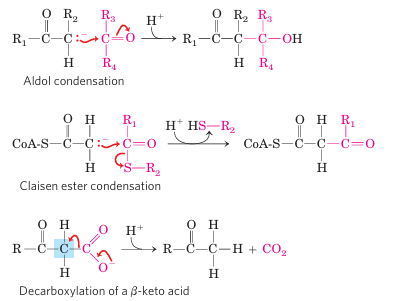
\includegraphics[width=0.7\textwidth]{build carbons}
	\caption{make or break carbon–carbon bonds}
\end{figure}

\paragraph{Internal rearrangements, Isomerizations, and Eliminations}
In this type of reactions \textbf{electrons are redistributed altering the bonding framework} without changing the overall oxidation state of the molecule. For example different groups undergo oxidation-reduction leading to \textbf{cis-trans rearrangements} or shifting the \textbf{position of double bonds} , i.e. formation of glucose 6-phosphate in glycolysis. Here C1 is reduced and C2 is oxidized. 
\begin{figure}[H]
	\centering
	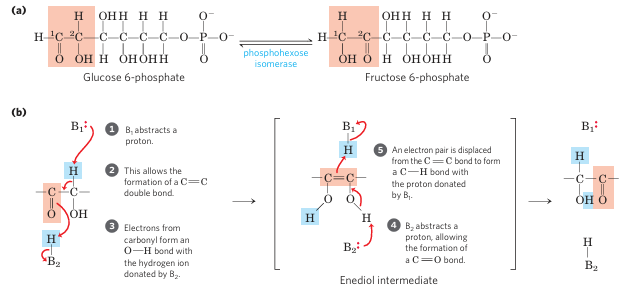
\includegraphics[width=0.7\textwidth]{changeposition}
	\caption{Isomerization and elimination reactions}
\end{figure}
En example for an \textbf{elimination} reaction is the loss of water from an alcohol resulting gin a double C=C bond. \textit{Similar reaction can result from eliminations in amines.}

\paragraph{Free-Radical Reactions}
The homolytic cleavage of covalent bonds generate free radicals. These radicals can then trigger other rations.   
\begin{figure}[H]
	\centering
	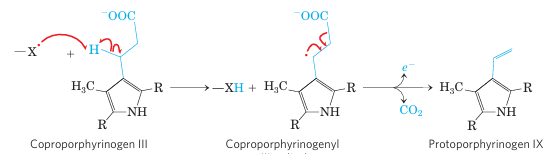
\includegraphics[width=0.7\textwidth]{radicals}
	\caption{A free radical–initiated decarboxylation reaction}
\end{figure}

\paragraph{Group Transfer Reactions}
The transfer of acyl, glycosyl, and phosphoryl groups from one nucleophile to another is common in living cells. \\
Acyl group transfer generally involves the addition of a nucleophile to the carbonyl carbon of an acyl group to form a tetrahedral intermediate.  \\
\\
A general idea in metabolism is to attach a good leaving group to a metabolic intermediate to trigger subsequent reactions. Since nucleophilic substitutions is made more favorable by the attachment of a phophoryl group to an otherwise poor leaving group such as -OH. \\

\begin{RemarkWithTitel}{Good leaving group}
	Recall that \textbf{weaker bases are better leaving groups}. On has to look how could the leaving group stabilize / balance the negative charge: 
	\textbf{Inorganic orthophosphate} (the ionized form of H\textsubscript{3}PO\textsubscript{4} at neutral pH, a mixture of H\textsubscript{2}PO\textsubscript{4}$^-$ and HPO\textsubscript{4}$^{2-}$, commonly abbreviated as \( \text{P}_i \)) and inorganic pyrophosphate (P\textsubscript{2}O\textsubscript{7}$^{4-}$, abbreviated as \( \text{PP}_i \)); \textbf{esters and anhydrides of phosphoric acid} and \textbf{thiols} are also good leaving groups. 
\end{RemarkWithTitel}

\begin{figure}[h]
	\centering
	\subfigure[Nucleophilic substitution]{
		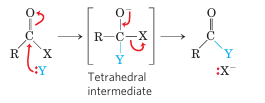
\includegraphics[width=0.45\textwidth]{group transfer}
	}
	\hfill
	% Second subfigure
	\subfigure[Rlative reactivity of carboxylic acid derivatives]{
		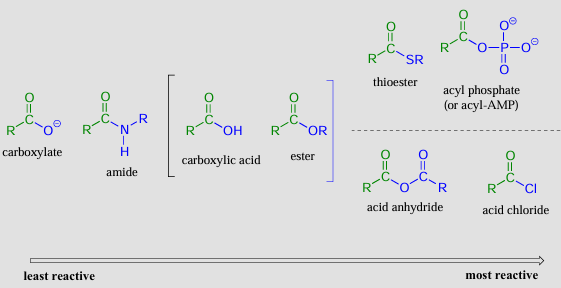
\includegraphics[width=0.5\textwidth]{reactivity}
		\label{reactivity}
	}
	\caption{Group Transfer Reactions}
\end{figure}


\paragraph{Oxidation-Reduction Reactions}
Carbon atoms can only exist in five oxidation states, depending on their binding partners. Note that \textbf{carbon is less electronegative than all atomes it is bound to, except hydrogen}. Thus all atoms that bind to carbon oxidaize it except hydrogen and therefore removing a hydrogen and replacing that bond with any other atom (including carbon) is synonymous with oxydation. Recall that every oxidation must be linked to a reduction. Note that, \textbf{Oxydations generally release energy} (camp fires where wood is ocidized). \\
\\
Often in biological oxidations, a compound loses two electrons and two hydrogens (2 hydrogen atoms), these reactions are called \textbf{dehydrogenations} catalized by \textbf{\gls{dehydrogenase}}. \\
\\
Sometimes in biological oxidations a carbon becomes covalently bounded to a oxygen. The corresponding enzymes are called \textbf{\gls{oxidase}} and if the oxygen atom is derived from molecular oxygen they are called \textbf{\gls{oxygenase}}. 

\begin{figure}[h]
	\centering
	\subfigure[The 5 oxidation levels of carbons]{
		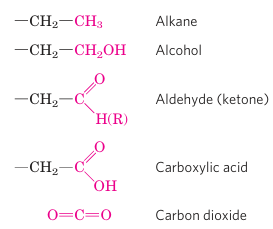
\includegraphics[width=0.4\textwidth]{oxidation_levels}
	}
	\hfill
	% Second subfigure
	\subfigure[lactate dehydrogenase]{
		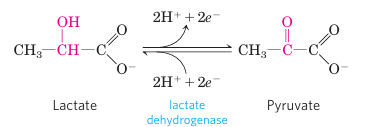
\includegraphics[width=0.5\textwidth]{lactat_deh}
	}
	\caption{Oxidation-Reduction Reactions}
\end{figure}


\subsection{Phosphoryl and ATP fun}
In a phosphate transfer reaction, a phosphate group is transferred from a phosphate group donor molecule to a phosphate group acceptor molecule.
\paragraph{Posphate groups}
Recall some important properties of phosporus from organic chemistry: 
\begin{itemize}
	\item Phosphates are \textbf{excellent leaving groups} in biological organic reactions, which can be seen for example in the hydrolysis of ATP.
	\item Phosphoric acid (H3PO4) is triprotonic, meaning that it has three acidic protons availble to donate with pKa values of 1, 6.5, 13, respectivly.
	\item Phosphorus can break the octet rule because it is in the third row of the periodic table and thus has \textbf{d orbitals} available for bonding. 
	\item The phosphate group is really tetrahedral, the \textbf{negative charges are delocalized} over the non-bridging oxygens, and there is some degree of protonation at physiological pH (with the exeption of the phosphate di-ester group.)
\end{itemize}

Phosphate transfer enzymes generally contain a \textbf{Mg2+ ion bound in the active site} in a position where it can interact with non-binding phophate oxygens on the substrate. This magnesium ion pulls the electron density away from the phosphorus atom, making it more electophilc. \\
\\
A phosphate transfer reaction can be thought of as a SN2 reaction at a carbon center. Recall that the phosphorus can form a "\textbf{5-bond}" \textbf{tranistion state}.


\paragraph{The phosphate enzymes}
\begin{DefWithTitle}{Kinases}
	\gls{kinase} (from Greek kinein, "to move") is an enzyme that catalyzes the transfer of phosphate groups from high-energy donor molecules, such as ATP, to specific substrates, a process known as phosphorylation.
\end{DefWithTitle}
\begin{DefWithTitle}{Phosphatases}
	\gls{phosphatase} is an enzyme that removes phosphate groups from proteins or other molecules, a process known as dephosphorylation, which often regulates cellular activity.
\end{DefWithTitle}
\begin{RemarkWithTitel}{Reactions catalyzed by kinases an phosphatases are \underline{not} the reverse of one another}
	Kinases irreversible transfer phopshate groups from ATP (or sometimes other nucleoside triphosphates) to various organic acceptors compounds, while phophatases tranfer phosphate from organic compunds to water: this are hydrolysis reactions. Kinase reactions involve an inherently "uphill" step (phosphorylation of alcohols for example) being paid with an inherently "downhill" step (cleavage of an anhydride bond in ATP). Phosphatase reactions, on the other hand, are thermodynamically "downhill", and while they require an enzyme to speed them up, they do not involve "spending" energy current the way kinases do. 
\end{RemarkWithTitel} 

\paragraph{ATP}
\textbf{\gls{atp}} is the the \textbf{energy currency} of the cell and links catabolism and anabolism. ATP is a high energy compund which can be seen when considering hydrolysis of ATP (highly exergonic), since: 
\begin{itemize}
	\item Hydrolysis relieves electrostatic repulsion between the negatively charged phosphates. One way to picture this is a\textbf{coil springing open, releasing potential energy}
	\item Inorganic phosphate can be stabilized by resonance hybride. 
	\item ADP-2 con ionize
	\item The products are better solvated than the reactants. 
\end{itemize} 
\textbf{Note:} that ATP-cleaving reaction are exothermic, but also have a high energy barrier, making it them very slow unless catalyzed by an enzyme. This helps us gain a tight control over the reactions in our metabolic pathways. \\
\\
\textbf{ATP provide energy by transferring its phosphate group and not by mere hydrolysis.} Nevertheless often we say that a given reaction is coupled to ATP hydrolysis which provides the energy required for the reaction to happen. Note that \textbf{ATP hydrolysis per se only provides heat.}\\
In many reactions \textbf{ATP is used as a phosphate donor} to a substrate that, once phosphorylated, acquires an higher free energy. 

\begin{figure}[H]
	\centering
	\subfigure[ATP hydrolysis]{
		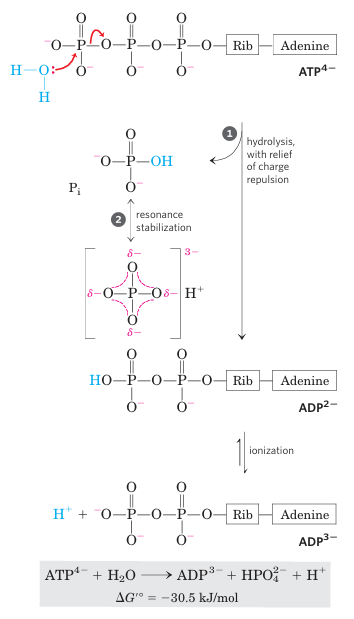
\includegraphics[width=0.25\textwidth]{atp_4}
		\label{atp_hydrolysis}
	}
	\subfigure[ATP provides energy]{
		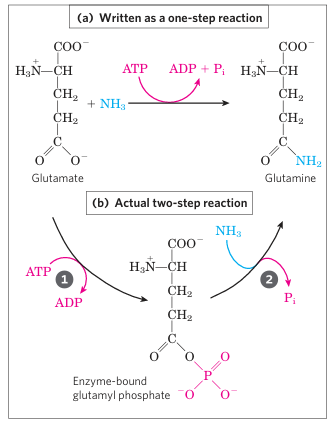
\includegraphics[width=0.25\textwidth]{atp_2}
		\label{atp_prov_energ}
	}
	\subfigure[ATP attack]{
		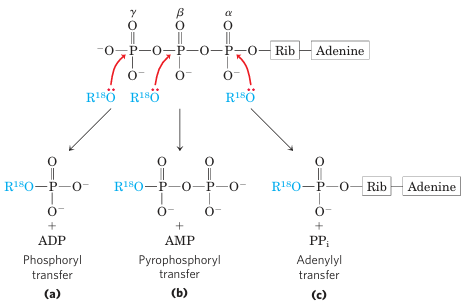
\includegraphics[width=0.4\textwidth]{atp_3}
		\label{ATP attack}
	}
	\caption{ATP}
	\label{atp}
\end{figure}

Note: To maintain its high group transfer potential, ATP concentration must be held far above the equilibrium concentration by energy-yielding reactions of catabolism.\\
Moreover, inorganic polyphosphate, present in all cells, may serve as a reservoir of phosphoryl groups with high group transfer potential. \\
\\
\textbf{To produce ATP we need higher energy compounds}. Cells contain other metabolites with large, negative, free energies of hydrolysis, including phosphoenolpyruvate, 1,3-bisphosphoglycerate, and phosphocreatine. These high-energy compounds, like ATP, have a high phosphoryl group transfer potential. Thioesters also have high free energies of hydrolysis.
\begin{figure}[H]
	\centering
	\subfigure[High energy phosphorylated compounds]{
		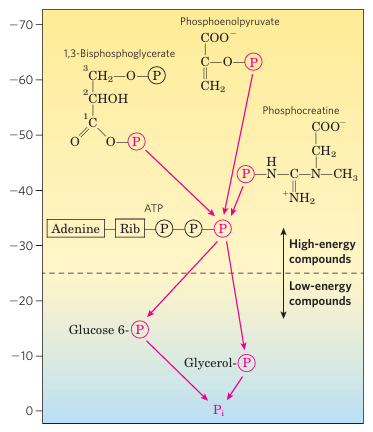
\includegraphics[width = 0.4\textwidth]{atp_1}
	}
	\subfigure[Standard free energies of Hydrolysis]{
		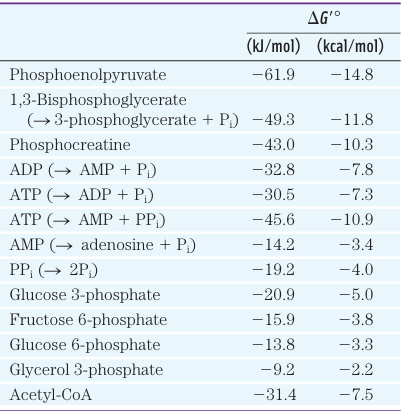
\includegraphics[width = 0.4\textwidth]{atp_6}
	}
	\caption{Hydrolysis of Phosphate compounds}
\end{figure}

\begin{RemarkWithTitel}{\gls{arsenatepoisoning}}
	A toxic condition caused by exposure to arsenate (AsO$_4^{3-}$), which disrupts cellular metabolism by \textbf{mimicking inorganic phosphate}. Arsenate can uncouple oxidative phosphorylation by substituting for inorganic phosphate oxidative pathways, ATP synthesis, leading to decreased ATP production and cellular toxicity.\\
	For example In the presence of arsenate, the product of glyceraldehyde 3-phosphate dehydrogenase is 1-arseno-3-phosphoglycerate, which nonenzymatically decomposes to 3-phosphoglycerate and arsenate; this substrate for the phosphoglycerate kinase is therefore bypassed, which leads in no net glycolytic synthesis of ATP.
\end{RemarkWithTitel}

\subsection{Biological Oxidation-Reduction Reactions}
Since we need high energy compounds to produce ATP. We have to ask us but how do we produce these Hi-NRG (NRG = energy)? -\textbf{The flow of electrons can do it!} 
\begin{DefWithTitle}{Electromotive force (emf)}
	Electrons flow from a reducing agent to an oxidizing agent due to their different electron affinities. This difference in affinities is called the electromotive force. Note that the reducing agent undergoes oxidation and the oxidizing agent undergoes reduction. 
\end{DefWithTitle}
\noindent Note, that \textbf{living cells have an biological "circuit", with a relatively reduced compound such as glucose as the source of electrons}. As glucose is enzymatically oxidized, the released electrons flow spontaneously through a series of electron-carrier intermediates to another chemical species, such as O2. This \textbf{electron flow is exergonic}, because O2 has a higher affinity for electrons than do the electron-carrier intermediates. This is exploited by the \textbf{ATP synthase} in the inner mitochondrial membrane that uses the proton-motive force to do chemical work. 

\paragraph{Dehydrogenation = Oxidation}
Dehydroganation corresponds to oxidation, since the carbon is less electronegative tha all atoms it is bound to except hydrogen. \textit{Note that not all oxidation-reduction reactions involve carbon, i.e conversion from nitrogen to ammonia.}\\
\\
There are different types electrons can be transfered: Directely as electrons, As hydrogen atoms, as a hydrogen ion or through direct combination with oxygen. Since all of this 4 types occur biologically the term \textbf{\gls{reducingequivalent}} is used.
 
\begin{figure}[H]
	\centering
	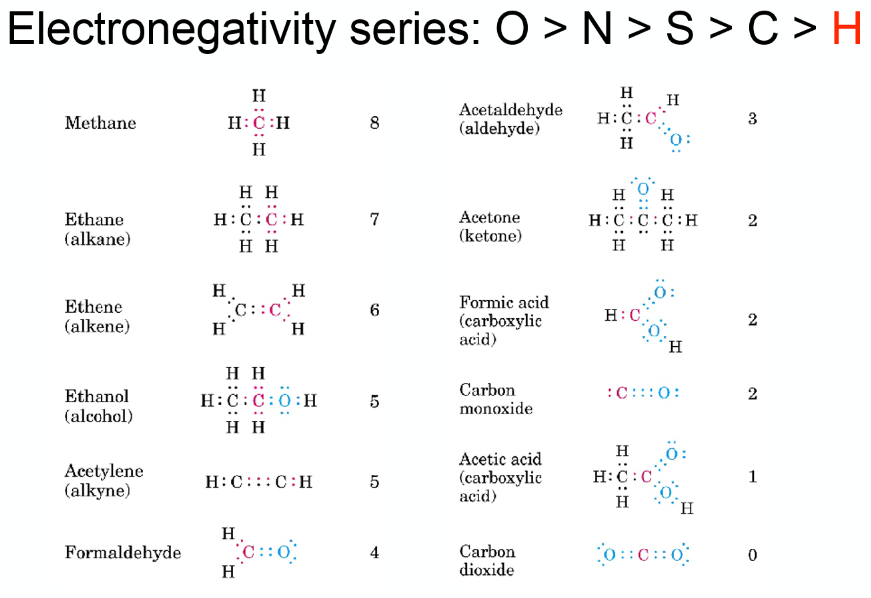
\includegraphics[width=0.7\textwidth]{reduction}
	\caption{Oxidation levels of a carbon compound in the biosphere}
\end{figure}

\subsection{Electron Carriers}
There are a multitude of enzymes that catalyze oxidation reactions from a variety of substrates, but most electrons end up in a \textbf{small set of univalve electron carriers}, such as NAD+, FAD, and Q (ubiquionel).  

\begin{DefWithTitle}{Electron Carriers}
	\gls{electroncarrier} are Molecules that can accept and donate electrons, facilitating the transfer of energy in redox reactions (e.g., NAD+, FAD).
\end{DefWithTitle}

\paragraph{NADH and NADPH}
These \textbf{watersolubable} coenzymes (\textit{\gls{nad} and \gls{nadp}}) can undergo \textbf{reversible reduction of the necotinamide ring}, as a substrate undergoes oxidation (dehydrogenation) giving up \textbf{2 hydrogen atoms}.
\begin{itemize}
	\item NAD+ and NADP+ take \textbf{2 electrons and 1 proton} while the second proton is released into solution. 
\end{itemize}
In many cells and tissues, the ratio of  NAD+ (oxidized) to NADH (reduced) is high, favoring hydride transfer from a substrate to NAD+ to form NADH. By contrast, NADPH is generally present at a higher concentration than NADP+, favoring hydride transfer from NADPH to a substrate. \\
\\
This reflects the specialized metabolic roles of the two coenzymes:\textbf{ NAD+ generally functions in oxidations—usually as part of a catabolic reaction}; \textbf{NADPH is the usual coenzyme in reductions—nearly always as part of an anabolic reaction}.

\begin{figure}[H]
	\centering
	\subfigure[NAD (a) and NADP (b)]{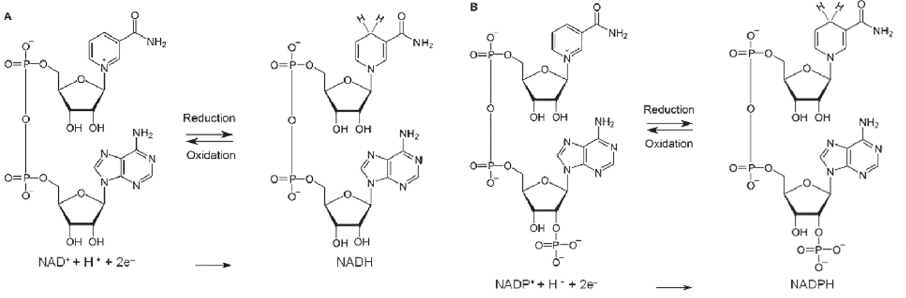
\includegraphics[width = 0.7\textwidth]{NAD_2}}
	\subfigure[Rossmann fold]{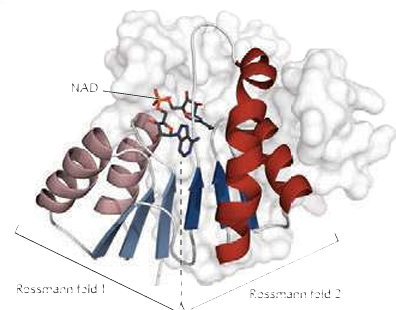
\includegraphics[width = 0.25 \textwidth]{NAD_1}}
	\caption{NADH and NADPH}
\end{figure}

\begin{RemarkWithTitel}{Dietary Deficiency of Niacin (Vitamin B3) cause Pellagra}
	NAD and NADP are derived from the \gls{niacin}), which is synthesized from tryptophan. Humans do generally not sysnthesize sufficient quantities of nacine, and this is especially so for individuals with diests low in tryptophan (diets based on maize for example). This leads to the disease pellagra. \\
	But note since NAD+ is can oxidize many thousands of molecules of glucose, since it the reduction always can be reversed. It is not necessarily to consume a lot of the vitamin, in contrary to glucose for example.  
\end{RemarkWithTitel}


\paragraph{FAD and FNM}
\gls{fad} and \gls{fmn} are coenzymes that are used in oxidation-reduction reactions by \textbf{\gls{flavoprotein}}. They are \textbf{tightly bound to their enzymes}, in contrast to NAD and NATP. Moreover, because flavin nucleotides can also only one electron and one proton taking on the partially reduced form. 
\begin{itemize}
	\item FAD and FNM take \textbf{1 or 2 electrons and 1or 2 protons} and remain tighly linked to the enzyme.
\end{itemize}
 Moreover, because flavin nucleotides can also \textbf{only one electron and one proton} taking on the partially reduced form. This is important since FAD and FMN are \textbf{key in electron transport reactions} (e.g. \textbf{ETC Complex I and II}), where electrons are passed one at a time. 

\begin{figure}[H]
	\centering
	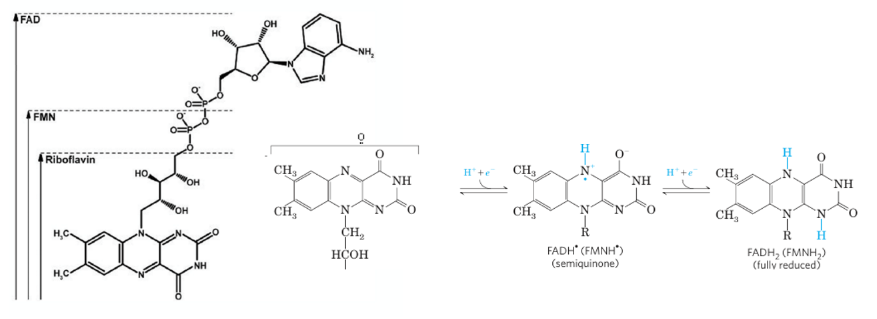
\includegraphics[width = 0.9 \textwidth]{FAD}
	\caption{Flavin Nucleotides}
\end{figure}
These Flavin nucleotides are derived from the \textbf{vitamin riboflavin} (B2)

\paragraph{Ubiquinone, Q}
\gls{ubiquinone} is a \textbf{lipid-soluble} electron carrier in the electron transport chain, transferring electrons between complex I/II and complex III. Ubiquinone exists in oxidized (Q), semiquinone (Q$^-$), and reduced (QH$_2$) forms.

\section{Metabolism}
Metabolism is the sum of all biochemical reactions in a living organism. The metabolism can be divided into two main pathways: catabolism and anabolism. 

\subsection{Catabolism <=> Anabolism}
\textbf{\gls{catabolism}} from greek meaning "\textbf{breaking down}" (Kata refers to down and bolë means to throw) is the process of breaking down complex molecules into simpler ones, \textbf{releasing/ producing energy in the form of ATP}. Examples include glycolysis, the Krebs cycle, and oxidative phosphorylation, which break down glucose and fatty acids to produce ATP. \textit{Note this catabolic pathways are mostly \textbf{converging}} \\
\\
In contrast, \textbf{\gls{anabolism}} from Greek meaning "\textbf{building up}" (Ana means up or again) is the synthesis of complex molecules from simpler ones, \textbf{requiring energy}. This process is essential for growth, repair, and maintenance of cells. Examples include protein synthesis, DNA replication, and lipid biosynthesis. \textit{Note this anabolic pathways are mostly \textbf{diverging}} 

\begin{figure}[H]
	\centering
	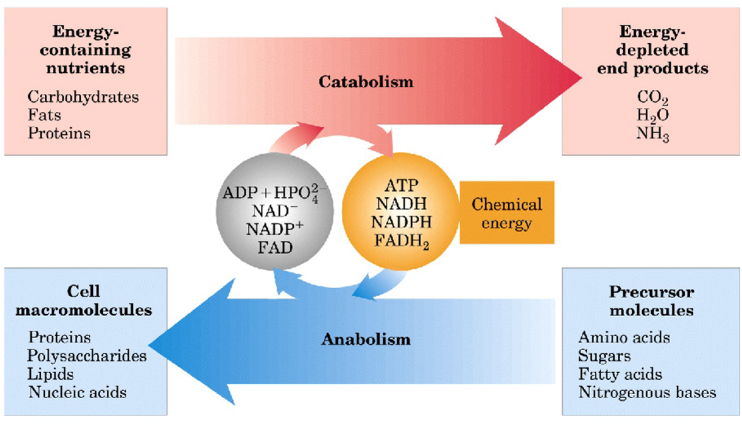
\includegraphics[width=0.7\textwidth]{cata_ana}
	\caption{Catabolism <=> Anabolism}
\end{figure}

\begin{figure}[H]
	\centering
	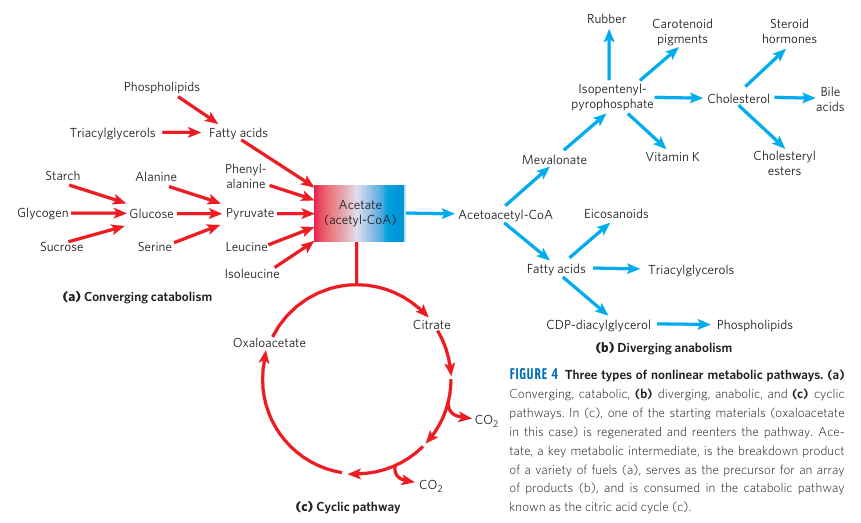
\includegraphics[width=0.8\textwidth]{pathways}
	\caption{Three types of nonlinear metabolic pathways}
\end{figure}


\subsection{Thermodynamic in Biological pathways}
\begin{DefWithTitle}{The second law of thermodynamics}
	The \gls{secondlaw} states that the total entropy of an isolated system can never decrease over time. Isolated systems spontaneously evolve toward thermodynamic equilibrium, the sate with the \textbf{maximum \gls{entropy}}.
\end{DefWithTitle}
In a \textbf{chemical reaction} entropy increases when the products of the reaction are less complex and more disordered than its substrates. Therefore in many biochemical reactions seam to contradict the second law as they "produce order"\\
To compensate the produced order by cells in their growth and division \textbf{free energy} is taken from the environment in the form of nutrients or solar light and exchanged for heat and entropy.
 
\begin{DefWithTitle}{Free energy (G)}
	In biochemistry, Gibbs free energy (\(G\)) determines whether a metabolic reaction "can occur spontaneously" (but may still be unlikely because of TS) in living systems. A process is favorable if it is \textbf{\gls{exergonicreaction}}, \(\Delta G < 0\). \\
	\\
	It represents the energy available to do biological work, such as muscle contraction, active transport, and biosynthesis.The change in Gibbs free energy (\(\Delta G\)) for a reaction is given by:
	\[
	\Delta G = \Delta H - T \Delta S
	\]
\end{DefWithTitle} 
An important property is that variations in delta G are \textbf{additive}:
\[
\Delta G_{\text{total}} = \Delta G_1 + \Delta G_2
\]
This property lets us \textbf{make unfavorable reaction favorable when coupling them to a highly favorable reaction}. These \textbf{\gls{coupledreactions}} are explored by various biological pathways.


%\printglossaries
\end{document}
